\documentclass[twoside]{book}

% Packages required by doxygen
\usepackage{fixltx2e}
\usepackage{calc}
\usepackage{doxygen}
\usepackage[export]{adjustbox} % also loads graphicx
\usepackage{graphicx}
\usepackage[utf8]{inputenc}
\usepackage{makeidx}
\usepackage{multicol}
\usepackage{multirow}
\PassOptionsToPackage{warn}{textcomp}
\usepackage{textcomp}
\usepackage[nointegrals]{wasysym}
\usepackage[table]{xcolor}

% Font selection
\usepackage[T1]{fontenc}
\usepackage[scaled=.90]{helvet}
\usepackage{courier}
\usepackage{amssymb}
\usepackage{sectsty}
\renewcommand{\familydefault}{\sfdefault}
\allsectionsfont{%
  \fontseries{bc}\selectfont%
  \color{darkgray}%
}
\renewcommand{\DoxyLabelFont}{%
  \fontseries{bc}\selectfont%
  \color{darkgray}%
}
\newcommand{\+}{\discretionary{\mbox{\scriptsize$\hookleftarrow$}}{}{}}

% Page & text layout
\usepackage{geometry}
\geometry{%
  a4paper,%
  top=2.5cm,%
  bottom=2.5cm,%
  left=2.5cm,%
  right=2.5cm%
}
\tolerance=750
\hfuzz=15pt
\hbadness=750
\setlength{\emergencystretch}{15pt}
\setlength{\parindent}{0cm}
\setlength{\parskip}{0.2cm}
\makeatletter
\renewcommand{\paragraph}{%
  \@startsection{paragraph}{4}{0ex}{-1.0ex}{1.0ex}{%
    \normalfont\normalsize\bfseries\SS@parafont%
  }%
}
\renewcommand{\subparagraph}{%
  \@startsection{subparagraph}{5}{0ex}{-1.0ex}{1.0ex}{%
    \normalfont\normalsize\bfseries\SS@subparafont%
  }%
}
\makeatother

% Headers & footers
\usepackage{fancyhdr}
\pagestyle{fancyplain}
\fancyhead[LE]{\fancyplain{}{\bfseries\thepage}}
\fancyhead[CE]{\fancyplain{}{}}
\fancyhead[RE]{\fancyplain{}{\bfseries\leftmark}}
\fancyhead[LO]{\fancyplain{}{\bfseries\rightmark}}
\fancyhead[CO]{\fancyplain{}{}}
\fancyhead[RO]{\fancyplain{}{\bfseries\thepage}}
\fancyfoot[LE]{\fancyplain{}{}}
\fancyfoot[CE]{\fancyplain{}{}}
\fancyfoot[RE]{\fancyplain{}{\bfseries\scriptsize Generated on Wed Dec 16 2015 08\+:12\+:43 for othello\+\_\+gr\+\_\+1\+\_\+5 by Doxygen }}
\fancyfoot[LO]{\fancyplain{}{\bfseries\scriptsize Generated on Wed Dec 16 2015 08\+:12\+:43 for othello\+\_\+gr\+\_\+1\+\_\+5 by Doxygen }}
\fancyfoot[CO]{\fancyplain{}{}}
\fancyfoot[RO]{\fancyplain{}{}}
\renewcommand{\footrulewidth}{0.4pt}
\renewcommand{\chaptermark}[1]{%
  \markboth{#1}{}%
}
\renewcommand{\sectionmark}[1]{%
  \markright{\thesection\ #1}%
}

% Indices & bibliography
\usepackage{natbib}
\usepackage[titles]{tocloft}
\setcounter{tocdepth}{3}
\setcounter{secnumdepth}{5}
\makeindex

% Hyperlinks (required, but should be loaded last)
\usepackage{ifpdf}
\ifpdf
  \usepackage[pdftex,pagebackref=true]{hyperref}
\else
  \usepackage[ps2pdf,pagebackref=true]{hyperref}
\fi
\hypersetup{%
  colorlinks=true,%
  linkcolor=blue,%
  citecolor=blue,%
  unicode%
}

% Custom commands
\newcommand{\clearemptydoublepage}{%
  \newpage{\pagestyle{empty}\cleardoublepage}%
}


%===== C O N T E N T S =====

\begin{document}

% Titlepage & ToC
\hypersetup{pageanchor=false,
             bookmarks=true,
             bookmarksnumbered=true,
             pdfencoding=unicode
            }
\pagenumbering{roman}
\begin{titlepage}
\vspace*{7cm}
\begin{center}%
{\Large othello\+\_\+gr\+\_\+1\+\_\+5 \\[1ex]\large 1.\+0 }\\
\vspace*{1cm}
{\large Generated by Doxygen 1.8.9.1}\\
\vspace*{0.5cm}
{\small Wed Dec 16 2015 08:12:43}\\
\end{center}
\end{titlepage}
\clearemptydoublepage
\tableofcontents
\clearemptydoublepage
\pagenumbering{arabic}
\hypersetup{pageanchor=true}

%--- Begin generated contents ---
\chapter{Data Structure Index}
\section{Structures de données}
Liste des structures de données avec une brève description \+:\begin{DoxyCompactList}
\item\contentsline{section}{\hyperlink{structCoup}{Coup} \\*Le type \hyperlink{structCoup}{Coup} permet de représenter le coup d\textquotesingle{}un joueur, en regroupant une position (sur le plateau) et un pion }{\pageref{structCoup}}{}
\item\contentsline{section}{\hyperlink{structCoups}{Coups} \\*Le type \hyperlink{structCoups}{Coups} permet de représenter un tableau de \hyperlink{structCoup}{Coup} et le nombre de \hyperlink{structCoup}{Coup} possibles }{\pageref{structCoups}}{}
\item\contentsline{section}{\hyperlink{structPion}{Pion} \\*Le type \hyperlink{structPion}{Pion} permet de représenter un pion }{\pageref{structPion}}{}
\item\contentsline{section}{\hyperlink{structPlateau}{Plateau} \\*Le type \hyperlink{structPlateau}{Plateau} permet de représenter un plateau }{\pageref{structPlateau}}{}
\item\contentsline{section}{\hyperlink{structPosition}{Position} \\*Le type \hyperlink{structPosition}{Position} permet de représenter une position sur le plateau }{\pageref{structPosition}}{}
\end{DoxyCompactList}

\chapter{File Index}
\section{File List}
Here is a list of all documented files with brief descriptions\+:\begin{DoxyCompactList}
\item\contentsline{section}{include/\hyperlink{_affichage_8h}{Affichage.\+h} \\*Fonctions d\textquotesingle{}affichage d\textquotesingle{}un plateau et d\textquotesingle{}affichage de l\textquotesingle{}aide }{\pageref{_affichage_8h}}{}
\item\contentsline{section}{include/\hyperlink{_faire_une_partie_8h}{Faire\+Une\+Partie.\+h} \\*Implantation de faireunepartie-\/prive pour le projet othello }{\pageref{_faire_une_partie_8h}}{}
\item\contentsline{section}{include/\hyperlink{_faire_une_partie___prive_8h}{Faire\+Une\+Partie\+\_\+\+Prive.\+h} \\*Implantation de faireunepartie-\/prive pour le projet othello }{\pageref{_faire_une_partie___prive_8h}}{}
\item\contentsline{section}{include/\hyperlink{_liste_coups_possibles_8h}{Liste\+Coups\+Possibles.\+h} \\*Implantation et signatures des fonctions publiques de Liste\+Coups\+Possibles }{\pageref{_liste_coups_possibles_8h}}{}
\item\contentsline{section}{include/{\bfseries Liste\+Coups\+Possibles\+\_\+\+Prive.\+h} }{\pageref{_liste_coups_possibles___prive_8h}}{}
\item\contentsline{section}{include/\hyperlink{_obtenir_coup_humain_8h}{Obtenir\+Coup\+Humain.\+h} \\*Implantation et signatures des fonctions publiques d\textquotesingle{}Obtenir\+Coup\+Humain }{\pageref{_obtenir_coup_humain_8h}}{}
\item\contentsline{section}{include/\hyperlink{_obtenir_coup_i_a_8h}{Obtenir\+Coup\+I\+A.\+h} \\*Implantation et signatures des fonctions publiques d\textquotesingle{}Obtenir\+Coup\+I\+A }{\pageref{_obtenir_coup_i_a_8h}}{}
\item\contentsline{section}{include/{\bfseries Obtenir\+Coup\+I\+A\+\_\+\+Prive.\+h} }{\pageref{_obtenir_coup_i_a___prive_8h}}{}
\item\contentsline{section}{include/\hyperlink{_t_a_d___couleur_8h}{T\+A\+D\+\_\+\+Couleur.\+h} \\*Implantation du T\+A\+D Couleur }{\pageref{_t_a_d___couleur_8h}}{}
\item\contentsline{section}{include/\hyperlink{_t_a_d___coup_8h}{T\+A\+D\+\_\+\+Coup.\+h} \\*Implantation du T\+A\+D \hyperlink{struct_coup}{Coup} }{\pageref{_t_a_d___coup_8h}}{}
\item\contentsline{section}{include/\hyperlink{_t_a_d___coups_8h}{T\+A\+D\+\_\+\+Coups.\+h} \\*Implantation du T\+A\+D \hyperlink{struct_coups}{Coups} }{\pageref{_t_a_d___coups_8h}}{}
\item\contentsline{section}{include/{\bfseries T\+A\+D\+\_\+\+Pion.\+h} }{\pageref{_t_a_d___pion_8h}}{}
\item\contentsline{section}{include/{\bfseries T\+A\+D\+\_\+\+Plateau.\+h} }{\pageref{_t_a_d___plateau_8h}}{}
\item\contentsline{section}{include/{\bfseries T\+A\+D\+\_\+\+Position.\+h} }{\pageref{_t_a_d___position_8h}}{}
\end{DoxyCompactList}

\chapter{Data Structure Documentation}
\hypertarget{struct_coup}{\section{Référence de la structure Coup}
\label{struct_coup}\index{Coup@{Coup}}
}


Le type \hyperlink{struct_coup}{Coup} permet de représenter le coup d'un joueur, en regroupant une position (sur le plateau) et un pion.  




{\ttfamily \#include $<$T\-A\-D\-\_\-\-Coup.\-h$>$}

\subsection*{Champs de données}
\begin{DoxyCompactItemize}
\item 
\hyperlink{struct_position}{Position} \hyperlink{struct_coup_a4d84949a19a29d3bb4dd2635c8241a83}{position}
\item 
\hyperlink{struct_pion}{Pion} \hyperlink{struct_coup_ad71b3ad38e648f9979a7e37f3ac0c258}{pion}
\end{DoxyCompactItemize}


\subsection{Description détaillée}
Le type \hyperlink{struct_coup}{Coup} permet de représenter le coup d'un joueur, en regroupant une position (sur le plateau) et un pion. 

\subsection{Documentation des champs}
\hypertarget{struct_coup_ad71b3ad38e648f9979a7e37f3ac0c258}{\index{Coup@{Coup}!pion@{pion}}
\index{pion@{pion}!Coup@{Coup}}
\subsubsection[{pion}]{\setlength{\rightskip}{0pt plus 5cm}{\bf Pion} pion}}\label{struct_coup_ad71b3ad38e648f9979a7e37f3ac0c258}
la hauteur de la grille \hypertarget{struct_coup_a4d84949a19a29d3bb4dd2635c8241a83}{\index{Coup@{Coup}!position@{position}}
\index{position@{position}!Coup@{Coup}}
\subsubsection[{position}]{\setlength{\rightskip}{0pt plus 5cm}{\bf Position} position}}\label{struct_coup_a4d84949a19a29d3bb4dd2635c8241a83}
la largeur de la grille 

La documentation de cette structure a été générée à partir du fichier suivant \-:\begin{DoxyCompactItemize}
\item 
include/\hyperlink{_t_a_d___coup_8h}{T\-A\-D\-\_\-\-Coup.\-h}\end{DoxyCompactItemize}

\hypertarget{struct_coups}{}\section{Coups Struct Reference}
\label{struct_coups}\index{Coups@{Coups}}


Le type \hyperlink{struct_coups}{Coups} permet de représenter un tableau de \hyperlink{struct_coup}{Coup} et le nombre de \hyperlink{struct_coup}{Coup} possibles.  




{\ttfamily \#include $<$T\+A\+D\+\_\+\+Coups.\+h$>$}



Collaboration diagram for Coups\+:
\nopagebreak
\begin{figure}[H]
\begin{center}
\leavevmode
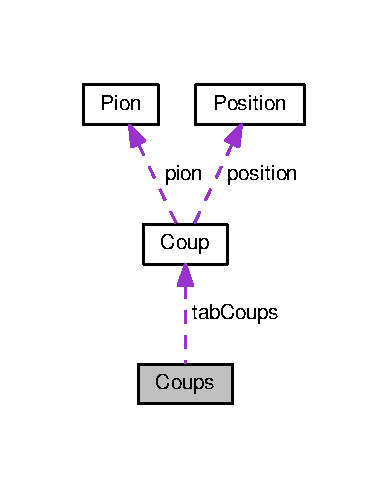
\includegraphics[width=186pt]{struct_coups__coll__graph}
\end{center}
\end{figure}
\subsection*{Data Fields}
\begin{DoxyCompactItemize}
\item 
\hypertarget{struct_coups_a7cea13a13332e303305612eb96861901}{}\hyperlink{struct_coup}{Coup} {\bfseries tab\+Coups} \mbox{[}M\+A\+X\+\_\+\+C\+O\+U\+P\+S\mbox{]}\label{struct_coups_a7cea13a13332e303305612eb96861901}

\item 
\hypertarget{struct_coups_a7e148eb1c2c883deb916170376c93d3c}{}unsigned int {\bfseries nb\+Cps}\label{struct_coups_a7e148eb1c2c883deb916170376c93d3c}

\end{DoxyCompactItemize}


\subsection{Detailed Description}
Le type \hyperlink{struct_coups}{Coups} permet de représenter un tableau de \hyperlink{struct_coup}{Coup} et le nombre de \hyperlink{struct_coup}{Coup} possibles. 

Definition at line 23 of file T\+A\+D\+\_\+\+Coups.\+h.



The documentation for this struct was generated from the following file\+:\begin{DoxyCompactItemize}
\item 
include/\hyperlink{_t_a_d___coups_8h}{T\+A\+D\+\_\+\+Coups.\+h}\end{DoxyCompactItemize}

\hypertarget{struct_pion}{}\section{Pion Struct Reference}
\label{struct_pion}\index{Pion@{Pion}}


Le type \hyperlink{struct_pion}{Pion} permet de représenter un pion.  




{\ttfamily \#include $<$T\+A\+D\+\_\+\+Pion.\+h$>$}

\subsection*{Data Fields}
\begin{DoxyCompactItemize}
\item 
\hyperlink{_t_a_d___couleur_8h_aa304d0ca681f782b1d7735da33037dd7}{Couleur} \hyperlink{struct_pion_af0e152d09c13944935e00bef7a3c5111}{couleur}
\end{DoxyCompactItemize}


\subsection{Detailed Description}
Le type \hyperlink{struct_pion}{Pion} permet de représenter un pion. 

Definition at line 19 of file T\+A\+D\+\_\+\+Pion.\+h.



\subsection{Field Documentation}
\hypertarget{struct_pion_af0e152d09c13944935e00bef7a3c5111}{}\index{Pion@{Pion}!couleur@{couleur}}
\index{couleur@{couleur}!Pion@{Pion}}
\subsubsection[{couleur}]{\setlength{\rightskip}{0pt plus 5cm}{\bf Couleur} couleur}\label{struct_pion_af0e152d09c13944935e00bef7a3c5111}
la couleur du pion 

Definition at line 20 of file T\+A\+D\+\_\+\+Pion.\+h.



The documentation for this struct was generated from the following file\+:\begin{DoxyCompactItemize}
\item 
include/T\+A\+D\+\_\+\+Pion.\+h\end{DoxyCompactItemize}

\hypertarget{struct_plateau}{\section{Référence de la structure Plateau}
\label{struct_plateau}\index{Plateau@{Plateau}}
}


Le type \hyperlink{struct_plateau}{Plateau} permet de représenter un plateau.  




{\ttfamily \#include $<$T\-A\-D\-\_\-\-Plateau.\-h$>$}

\subsection*{Champs de données}
\begin{DoxyCompactItemize}
\item 
\hyperlink{struct_pion}{Pion} \hyperlink{struct_plateau_aa14649bf1b37b316f42ffcb79c1951a5}{pions} \mbox{[}8\mbox{]}\mbox{[}8\mbox{]}
\item 
int \hyperlink{struct_plateau_a5df6e631fe34def5ff04a0b4dd233ae5}{presence\-Pions} \mbox{[}8\mbox{]}\mbox{[}8\mbox{]}
\end{DoxyCompactItemize}


\subsection{Description détaillée}
Le type \hyperlink{struct_plateau}{Plateau} permet de représenter un plateau. 

\subsection{Documentation des champs}
\hypertarget{struct_plateau_aa14649bf1b37b316f42ffcb79c1951a5}{\index{Plateau@{Plateau}!pions@{pions}}
\index{pions@{pions}!Plateau@{Plateau}}
\subsubsection[{pions}]{\setlength{\rightskip}{0pt plus 5cm}{\bf Pion} pions\mbox{[}8\mbox{]}\mbox{[}8\mbox{]}}}\label{struct_plateau_aa14649bf1b37b316f42ffcb79c1951a5}
les pions du plateau \hypertarget{struct_plateau_a5df6e631fe34def5ff04a0b4dd233ae5}{\index{Plateau@{Plateau}!presence\-Pions@{presence\-Pions}}
\index{presence\-Pions@{presence\-Pions}!Plateau@{Plateau}}
\subsubsection[{presence\-Pions}]{\setlength{\rightskip}{0pt plus 5cm}int presence\-Pions\mbox{[}8\mbox{]}\mbox{[}8\mbox{]}}}\label{struct_plateau_a5df6e631fe34def5ff04a0b4dd233ae5}
la case est remplie ou non \-: 0 si vide, 1 si remplie 

La documentation de cette structure a été générée à partir du fichier suivant \-:\begin{DoxyCompactItemize}
\item 
include/T\-A\-D\-\_\-\-Plateau.\-h\end{DoxyCompactItemize}

\hypertarget{struct_position}{}\section{Position Struct Reference}
\label{struct_position}\index{Position@{Position}}


Le type \hyperlink{struct_position}{Position} permet de représenter une position sur le plateau.  




{\ttfamily \#include $<$T\+A\+D\+\_\+\+Position.\+h$>$}

\subsection*{Data Fields}
\begin{DoxyCompactItemize}
\item 
unsigned int \hyperlink{struct_position_a90d401bbcd8cccd70cbe1b638ba239cf}{ligne}
\item 
unsigned int \hyperlink{struct_position_a62f746fce1dec24c5a8c5fa3f7a71bcd}{colonne}
\end{DoxyCompactItemize}


\subsection{Detailed Description}
Le type \hyperlink{struct_position}{Position} permet de représenter une position sur le plateau. 

Definition at line 18 of file T\+A\+D\+\_\+\+Position.\+h.



\subsection{Field Documentation}
\hypertarget{struct_position_a62f746fce1dec24c5a8c5fa3f7a71bcd}{}\index{Position@{Position}!colonne@{colonne}}
\index{colonne@{colonne}!Position@{Position}}
\subsubsection[{colonne}]{\setlength{\rightskip}{0pt plus 5cm}unsigned int colonne}\label{struct_position_a62f746fce1dec24c5a8c5fa3f7a71bcd}
l\textquotesingle{}indice\textquotesingle{} de la colonne du plateau 

Definition at line 20 of file T\+A\+D\+\_\+\+Position.\+h.

\hypertarget{struct_position_a90d401bbcd8cccd70cbe1b638ba239cf}{}\index{Position@{Position}!ligne@{ligne}}
\index{ligne@{ligne}!Position@{Position}}
\subsubsection[{ligne}]{\setlength{\rightskip}{0pt plus 5cm}unsigned int ligne}\label{struct_position_a90d401bbcd8cccd70cbe1b638ba239cf}
l\textquotesingle{}indice de la ligne du plateau 

Definition at line 19 of file T\+A\+D\+\_\+\+Position.\+h.



The documentation for this struct was generated from the following file\+:\begin{DoxyCompactItemize}
\item 
include/T\+A\+D\+\_\+\+Position.\+h\end{DoxyCompactItemize}

\chapter{File Documentation}
\hypertarget{_affichage_8h}{}\section{include/\+Affichage.h File Reference}
\label{_affichage_8h}\index{include/\+Affichage.\+h@{include/\+Affichage.\+h}}


Fonctions d\textquotesingle{}affichage d\textquotesingle{}un plateau et d\textquotesingle{}affichage de l\textquotesingle{}aide.  


{\ttfamily \#include \char`\"{}T\+A\+D\+\_\+\+Couleur.\+h\char`\"{}}\\*
{\ttfamily \#include \char`\"{}T\+A\+D\+\_\+\+Pion.\+h\char`\"{}}\\*
{\ttfamily \#include \char`\"{}T\+A\+D\+\_\+\+Plateau.\+h\char`\"{}}\\*
{\ttfamily \#include \char`\"{}T\+A\+D\+\_\+\+Position.\+h\char`\"{}}\\*
{\ttfamily \#include \char`\"{}T\+A\+D\+\_\+\+Coup.\+h\char`\"{}}\\*
Include dependency graph for Affichage.\+h\+:
\nopagebreak
\begin{figure}[H]
\begin{center}
\leavevmode
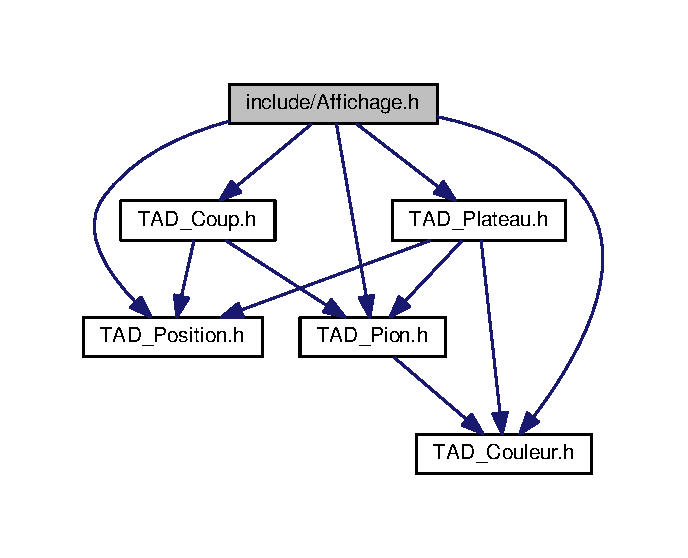
\includegraphics[width=330pt]{_affichage_8h__incl}
\end{center}
\end{figure}
\subsection*{Functions}
\begin{DoxyCompactItemize}
\item 
\hypertarget{_affichage_8h_a073375ed46d7f2d21c61262a5af52930}{}void \hyperlink{_affichage_8h_a073375ed46d7f2d21c61262a5af52930}{afficher\+Aide} ()\label{_affichage_8h_a073375ed46d7f2d21c61262a5af52930}

\begin{DoxyCompactList}\small\item\em Fonction qui affiche l\textquotesingle{}aide du jeu d\textquotesingle{}Othello (exécutable appelé sans argument) \end{DoxyCompactList}\item 
\hypertarget{_affichage_8h_af24e3ad5f898ceab9d3011cff1ff793a}{}void {\bfseries afficher\+Tournoi} (\hyperlink{struct_plateau}{Plateau} plateau, \hyperlink{struct_coup}{Coup} coup, int a\+Pu\+Jouer, int est\+Partie\+Finie)\label{_affichage_8h_af24e3ad5f898ceab9d3011cff1ff793a}

\item 
char \hyperlink{_affichage_8h_a797147b14780279afc9943eaac537888}{int\+To\+Char} (unsigned int i)
\begin{DoxyCompactList}\small\item\em Fonction qui convertit un entier en une lettre. \end{DoxyCompactList}\item 
\hypertarget{_affichage_8h_ae90e85a8322ed3a0b2e98d25a947dd35}{}void {\bfseries afficher\+Plateau} (\hyperlink{struct_plateau}{Plateau} plateau, \hyperlink{struct_coup}{Coup} coup, int a\+Pu\+Jouer, int est\+Partie\+Finie)\label{_affichage_8h_ae90e85a8322ed3a0b2e98d25a947dd35}

\end{DoxyCompactItemize}


\subsection{Detailed Description}
Fonctions d\textquotesingle{}affichage d\textquotesingle{}un plateau et d\textquotesingle{}affichage de l\textquotesingle{}aide. 

\begin{DoxyAuthor}{Author}
Groupe 1.\+5 
\end{DoxyAuthor}
\begin{DoxyVersion}{Version}
1.\+0 
\end{DoxyVersion}
\begin{DoxyDate}{Date}
09/12/2015 
\end{DoxyDate}


\subsection{Function Documentation}
\hypertarget{_affichage_8h_a797147b14780279afc9943eaac537888}{}\index{Affichage.\+h@{Affichage.\+h}!int\+To\+Char@{int\+To\+Char}}
\index{int\+To\+Char@{int\+To\+Char}!Affichage.\+h@{Affichage.\+h}}
\subsubsection[{int\+To\+Char}]{\setlength{\rightskip}{0pt plus 5cm}char int\+To\+Char (
\begin{DoxyParamCaption}
\item[{unsigned int}]{i}
\end{DoxyParamCaption}
)}\label{_affichage_8h_a797147b14780279afc9943eaac537888}


Fonction qui convertit un entier en une lettre. 


\begin{DoxyParams}{Parameters}
{\em unsigned} & int i, l\textquotesingle{}entier à convertir \\
\hline
\end{DoxyParams}
\begin{DoxyReturn}{Returns}
char 
\end{DoxyReturn}

\hypertarget{_faire_une_partie_8h}{\section{Référence du fichier include/\-Faire\-Une\-Partie.h}
\label{_faire_une_partie_8h}\index{include/\-Faire\-Une\-Partie.\-h@{include/\-Faire\-Une\-Partie.\-h}}
}


Implantation de faireunepartie-\/prive pour le projet othello.  


{\ttfamily \#include \char`\"{}Faire\-Une\-Partie\-\_\-\-Prive.\-h\char`\"{}}\\*
\subsection*{Fonctions}
\begin{DoxyCompactItemize}
\item 
void \hyperlink{_faire_une_partie_8h_a30385e641c6f3cc4be0064a153c42355}{faire\-Une\-Partie} (void($\ast$afficher\-Plateau)(\hyperlink{struct_plateau}{Plateau}, \hyperlink{struct_coup}{Coup}, int, int), \hyperlink{struct_coup}{Coup}($\ast$get\-Coup1)(\hyperlink{struct_plateau}{Plateau}, \hyperlink{_t_a_d___couleur_8h_aa304d0ca681f782b1d7735da33037dd7}{Couleur}), \hyperlink{struct_coup}{Coup}($\ast$get\-Coup2)(\hyperlink{struct_plateau}{Plateau}, \hyperlink{_t_a_d___couleur_8h_aa304d0ca681f782b1d7735da33037dd7}{Couleur}), \hyperlink{_t_a_d___couleur_8h_aa304d0ca681f782b1d7735da33037dd7}{Couleur} $\ast$vainqueur, int $\ast$est\-Match\-Nul, \hyperlink{_t_a_d___couleur_8h_aa304d0ca681f782b1d7735da33037dd7}{Couleur} couleur\-Joueur1)
\begin{DoxyCompactList}\small\item\em Faire\-Une\-Partie regroupe la procedure faire\-Une\-Partie qui va permettre de jouer a l'othello. \end{DoxyCompactList}\item 
void \hyperlink{_faire_une_partie_8h_a72253f5f7bcc8905865eb0bd84b7e726}{pion\-Est\-Present} (\hyperlink{struct_pion}{Pion} pion\-Joueur, \hyperlink{_faire_une_partie___prive_8h_a224b9163917ac32fc95a60d8c1eec3aa}{Direction} dir\-A\-Tester, \hyperlink{struct_position}{Position} $\ast$pos, \hyperlink{struct_plateau}{Plateau} $\ast$plateau, int $\ast$pion\-Present)
\begin{DoxyCompactList}\small\item\em Procedure qui permet de savoir si un pion est présent sur le plateau selon une direction, et si oui quelle est sa position. \end{DoxyCompactList}\item 
void \hyperlink{_faire_une_partie_8h_ad6602db9273ba66952c5b707b1b82b21}{nb\-Pions} (\hyperlink{struct_plateau}{Plateau} plateau, int $\ast$nb\-Pions\-Noirs, int $\ast$nb\-Pions\-Blancs)
\begin{DoxyCompactList}\small\item\em Procedure qui permet de compter le nombre de pions des joueurs 1 et 2 sur le plateau. \end{DoxyCompactList}\end{DoxyCompactItemize}


\subsection{Description détaillée}
Implantation de faireunepartie-\/prive pour le projet othello. \begin{DoxyAuthor}{Auteur}
groupe 1.\-5 
\end{DoxyAuthor}
\begin{DoxyVersion}{Version}
1.\-0 
\end{DoxyVersion}
\begin{DoxyDate}{Date}
02/12/2015 
\end{DoxyDate}


\subsection{Documentation des fonctions}
\hypertarget{_faire_une_partie_8h_a30385e641c6f3cc4be0064a153c42355}{\index{Faire\-Une\-Partie.\-h@{Faire\-Une\-Partie.\-h}!faire\-Une\-Partie@{faire\-Une\-Partie}}
\index{faire\-Une\-Partie@{faire\-Une\-Partie}!FaireUnePartie.h@{Faire\-Une\-Partie.\-h}}
\subsubsection[{faire\-Une\-Partie}]{\setlength{\rightskip}{0pt plus 5cm}void faire\-Une\-Partie (
\begin{DoxyParamCaption}
\item[{void($\ast$)({\bf Plateau}, {\bf Coup}, int, int)}]{afficher\-Plateau, }
\item[{{\bf Coup}($\ast$)({\bf Plateau}, {\bf Couleur})}]{get\-Coup1, }
\item[{{\bf Coup}($\ast$)({\bf Plateau}, {\bf Couleur})}]{get\-Coup2, }
\item[{{\bf Couleur} $\ast$}]{vainqueur, }
\item[{int $\ast$}]{est\-Match\-Nul, }
\item[{{\bf Couleur}}]{couleur\-Joueur1}
\end{DoxyParamCaption}
)}}\label{_faire_une_partie_8h_a30385e641c6f3cc4be0064a153c42355}


Faire\-Une\-Partie regroupe la procedure faire\-Une\-Partie qui va permettre de jouer a l'othello. 

faire\-Une\-Partie(void($<$em$>$afficher\-Plateau)(\hyperlink{struct_plateau}{Plateau}), \hyperlink{struct_coup}{Coup($\ast$get\-Coup)}(\hyperlink{struct_plateau}{Plateau},\hyperlink{struct_pion}{Pion}), \hyperlink{struct_coup}{Coup($\ast$get\-Coup)}(\hyperlink{struct_plateau}{Plateau},\hyperlink{struct_pion}{Pion}), Couleur vainqueur, int$\ast$ est\-Match\-Nul, Couleur couleur\-Joueur1) Procedure permettant de jouer au jeu de l'othello


\begin{DoxyParams}{Paramètres}
{\em void($\ast$afficher\-Plateau)(\-Plateau,\hyperlink{struct_coup}{Coup},int,int)} & P\-O\-I\-N\-T\-E\-U\-R sur une fonction qui permet d'afficher le plateau a chaque tour \\
\hline
{\em \hyperlink{struct_coup}{Coup($\ast$get\-Coup1)(\-Plateau},Pion)} & permet d'obtenir le coup du joueur 1 \\
\hline
{\em \hyperlink{struct_coup}{Coup($\ast$get\-Coup2)(\-Plateau},Pion)} & permet d'obtenir le coup du joueur 2 \\
\hline
{\em Couleur$\ast$} & vaiqueur permet de determiner le gagnant de la partie \\
\hline
{\em int$\ast$} & est\-Match\-Nul booléen qui permet de savoir si aucun joueur n'a gagné la partie ou il y'a un gagnant \\
\hline
{\em Couleur} & couleur\-Joueur1 permet d'obtenir la couleur choisie par le joueur 1 \textbackslash{} \\
\hline
\end{DoxyParams}
\hypertarget{_faire_une_partie_8h_ad6602db9273ba66952c5b707b1b82b21}{\index{Faire\-Une\-Partie.\-h@{Faire\-Une\-Partie.\-h}!nb\-Pions@{nb\-Pions}}
\index{nb\-Pions@{nb\-Pions}!FaireUnePartie.h@{Faire\-Une\-Partie.\-h}}
\subsubsection[{nb\-Pions}]{\setlength{\rightskip}{0pt plus 5cm}void nb\-Pions (
\begin{DoxyParamCaption}
\item[{{\bf Plateau}}]{plateau, }
\item[{int $\ast$}]{nb\-Pions\-Noirs, }
\item[{int $\ast$}]{nb\-Pions\-Blancs}
\end{DoxyParamCaption}
)}}\label{_faire_une_partie_8h_ad6602db9273ba66952c5b707b1b82b21}


Procedure qui permet de compter le nombre de pions des joueurs 1 et 2 sur le plateau. 

void nb\-Pions (\hyperlink{struct_plateau}{Plateau} plateau, unsigned int$\ast$ score\-Joueur1, unsigned int$\ast$ score\-Joueur2) 
\begin{DoxyParams}{Paramètres}
{\em \hyperlink{struct_plateau}{Plateau}} & plateau, le plateau de jeu \\
\hline
{\em int$\ast$} & nb\-Pions\-Blancs, le nombre de pions Blanc \\
\hline
{\em int$\ast$} & nb\-Pions\-Noirs, le nombre de pions Noirs \textbackslash{} \\
\hline
\end{DoxyParams}
\hypertarget{_faire_une_partie_8h_a72253f5f7bcc8905865eb0bd84b7e726}{\index{Faire\-Une\-Partie.\-h@{Faire\-Une\-Partie.\-h}!pion\-Est\-Present@{pion\-Est\-Present}}
\index{pion\-Est\-Present@{pion\-Est\-Present}!FaireUnePartie.h@{Faire\-Une\-Partie.\-h}}
\subsubsection[{pion\-Est\-Present}]{\setlength{\rightskip}{0pt plus 5cm}void pion\-Est\-Present (
\begin{DoxyParamCaption}
\item[{{\bf Pion}}]{pion\-Joueur, }
\item[{{\bf Direction}}]{dir\-A\-Tester, }
\item[{{\bf Position} $\ast$}]{pos, }
\item[{{\bf Plateau} $\ast$}]{plateau, }
\item[{int $\ast$}]{pion\-Present}
\end{DoxyParamCaption}
)}}\label{_faire_une_partie_8h_a72253f5f7bcc8905865eb0bd84b7e726}


Procedure qui permet de savoir si un pion est présent sur le plateau selon une direction, et si oui quelle est sa position. 

void pion\-Est\-Present(\-Pion pion\-Joueur, unsigned int x, unsigned int y, Position$\ast$ pos, Plateau$\ast$ plateau, int$\ast$ pion\-Present) 
\begin{DoxyParams}{Paramètres}
{\em \hyperlink{struct_pion}{Pion}} & pion\-Joueur, le pion représentant le joueur  \\
\hline
{\em Direction} & dir\-A\-Tester, la direction à tester \\
\hline
{\em Position$\ast$} & pos, la position initiale du pion qui, à la fin de l'exécution de la procédure, renvoit la position du pion trouvé \\
\hline
{\em Plateau$\ast$} & plateau, le plateau de jeu \\
\hline
{\em int$\ast$} & pion\-Present, qui renvoit 0 si aucun pion conforme n'a été trouvé, 1 sinon \textbackslash{} \\
\hline
\end{DoxyParams}

\hypertarget{_faire_une_partie___prive_8h}{}\section{include/\+Faire\+Une\+Partie\+\_\+\+Prive.h File Reference}
\label{_faire_une_partie___prive_8h}\index{include/\+Faire\+Une\+Partie\+\_\+\+Prive.\+h@{include/\+Faire\+Une\+Partie\+\_\+\+Prive.\+h}}


Implantation de faireunepartie-\/prive pour le projet othello.  


{\ttfamily \#include \char`\"{}T\+A\+D\+\_\+\+Plateau.\+h\char`\"{}}\\*
{\ttfamily \#include \char`\"{}T\+A\+D\+\_\+\+Couleur.\+h\char`\"{}}\\*
{\ttfamily \#include \char`\"{}T\+A\+D\+\_\+\+Position.\+h\char`\"{}}\\*
{\ttfamily \#include \char`\"{}T\+A\+D\+\_\+\+Pion.\+h\char`\"{}}\\*
{\ttfamily \#include \char`\"{}T\+A\+D\+\_\+\+Coup.\+h\char`\"{}}\\*
{\ttfamily \#include \char`\"{}T\+A\+D\+\_\+\+Coups.\+h\char`\"{}}\\*
{\ttfamily \#include \char`\"{}Faire\+Une\+Partie.\+h\char`\"{}}\\*
Include dependency graph for Faire\+Une\+Partie\+\_\+\+Prive.\+h\+:
\nopagebreak
\begin{figure}[H]
\begin{center}
\leavevmode
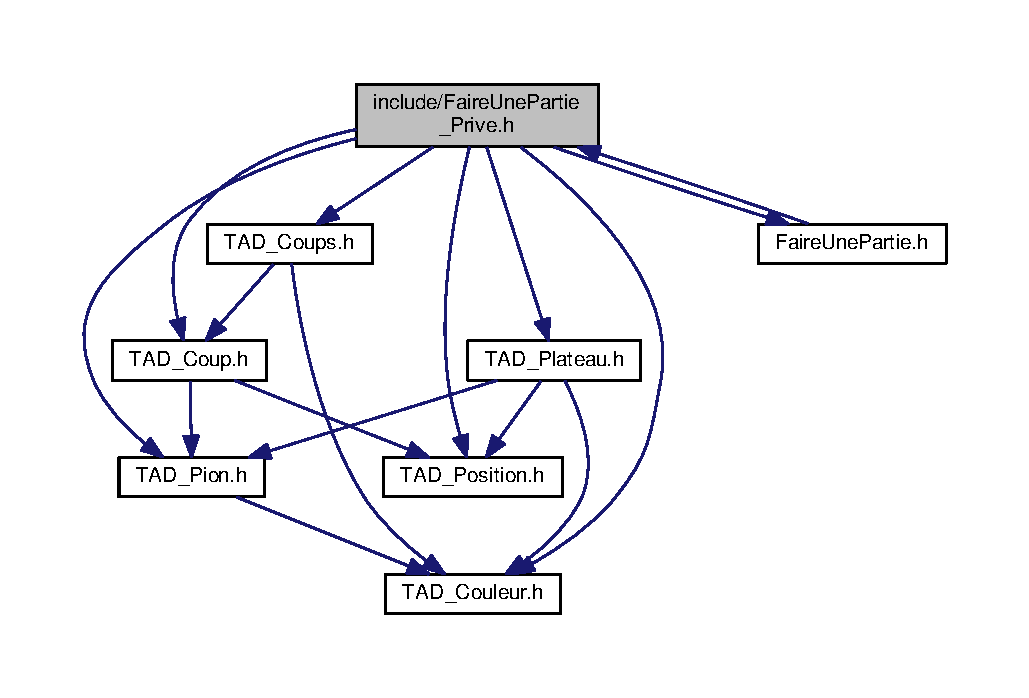
\includegraphics[width=350pt]{_faire_une_partie___prive_8h__incl}
\end{center}
\end{figure}
This graph shows which files directly or indirectly include this file\+:
\nopagebreak
\begin{figure}[H]
\begin{center}
\leavevmode
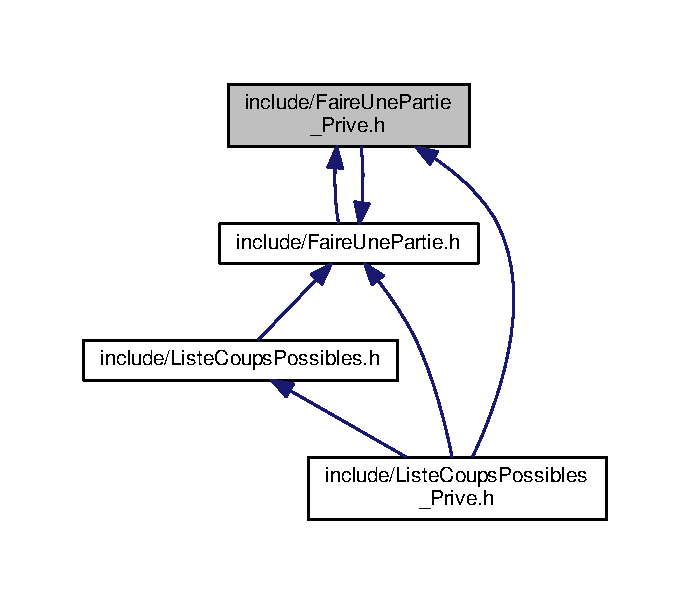
\includegraphics[width=331pt]{_faire_une_partie___prive_8h__dep__incl}
\end{center}
\end{figure}
\subsection*{Enumerations}
\begin{DoxyCompactItemize}
\item 
\hypertarget{_faire_une_partie___prive_8h_a224b9163917ac32fc95a60d8c1eec3aa}{}enum \hyperlink{_faire_une_partie___prive_8h_a224b9163917ac32fc95a60d8c1eec3aa}{Direction} \{ \\*
{\bfseries G\+A\+U\+C\+H\+E}, 
{\bfseries D\+R\+O\+I\+T\+E}, 
{\bfseries H\+A\+U\+T}, 
{\bfseries B\+A\+S}, 
\\*
{\bfseries D\+I\+A\+G\+G\+H}, 
{\bfseries D\+I\+A\+G\+G\+B}, 
{\bfseries D\+I\+A\+G\+D\+H}, 
{\bfseries D\+I\+A\+G\+D\+B}
 \}\label{_faire_une_partie___prive_8h_a224b9163917ac32fc95a60d8c1eec3aa}

\begin{DoxyCompactList}\small\item\em Faire\+Une\+Partie-\/prive regroupe seulement les fonctions et procédures qu\textquotesingle{}on va utiliser dans F\+A\+I\+R\+E\+U\+N\+E\+P\+A\+R\+T\+I\+E. \end{DoxyCompactList}\end{DoxyCompactItemize}
\subsection*{Functions}
\begin{DoxyCompactItemize}
\item 
\hypertarget{_faire_une_partie___prive_8h_aaf339dd563c8bdd5f02f1fc94d9295b7}{}\hyperlink{struct_position}{Position} {\bfseries D\+I\+R\+\_\+position\+Selon\+Direction} (\hyperlink{struct_position}{Position} pos\+Init, \hyperlink{_faire_une_partie___prive_8h_a224b9163917ac32fc95a60d8c1eec3aa}{Direction} dir\+Deplacement)\label{_faire_une_partie___prive_8h_aaf339dd563c8bdd5f02f1fc94d9295b7}

\item 
\hypertarget{_faire_une_partie___prive_8h_a14fba88b3696b98569655ed19a28b609}{}\hyperlink{_faire_une_partie___prive_8h_a224b9163917ac32fc95a60d8c1eec3aa}{Direction} {\bfseries D\+I\+R\+\_\+inverser\+Direction} (\hyperlink{_faire_une_partie___prive_8h_a224b9163917ac32fc95a60d8c1eec3aa}{Direction} dir\+Init)\label{_faire_une_partie___prive_8h_a14fba88b3696b98569655ed19a28b609}

\item 
\hypertarget{_faire_une_partie___prive_8h_aabcf85ca5155b18ac3e40e85f0d5b0bb}{}int {\bfseries D\+I\+R\+\_\+deplacement\+Valide} (\hyperlink{struct_position}{Position} pos, \hyperlink{_faire_une_partie___prive_8h_a224b9163917ac32fc95a60d8c1eec3aa}{Direction} dir\+Deplacement)\label{_faire_une_partie___prive_8h_aabcf85ca5155b18ac3e40e85f0d5b0bb}

\item 
void \hyperlink{_faire_une_partie___prive_8h_abef4802712cdf356b802706d2c0b97b6}{initialiser\+Plateau} (\hyperlink{struct_plateau}{Plateau} $\ast$plateau)
\begin{DoxyCompactList}\small\item\em Procedure permettant d\textquotesingle{}initialiser le plateau (place quatre pions au centre) \end{DoxyCompactList}\item 
void \hyperlink{_faire_une_partie___prive_8h_aa99d3a46026468b5043c9599414f10b2}{jouer} (\hyperlink{struct_plateau}{Plateau} $\ast$plateau, \hyperlink{_t_a_d___couleur_8h_aa304d0ca681f782b1d7735da33037dd7}{Couleur} $\ast$couleur\+Joueur, \hyperlink{struct_coup}{Coup}($\ast$obtenir\+Coup\+Joueur)(\hyperlink{struct_plateau}{Plateau}, \hyperlink{_t_a_d___couleur_8h_aa304d0ca681f782b1d7735da33037dd7}{Couleur}), int $\ast$a\+Pu\+Jouer, \hyperlink{struct_coup}{Coup} $\ast$coup\+Joueur)
\begin{DoxyCompactList}\small\item\em Procedure qui permet à un joueur de jouer. \end{DoxyCompactList}\item 
void \hyperlink{_faire_une_partie___prive_8h_aef0dc8a08a42ddf7c9b0cb7f657a95b6}{jouer\+Coup} (\hyperlink{struct_coup}{Coup} coup, \hyperlink{struct_plateau}{Plateau} $\ast$plateau)
\begin{DoxyCompactList}\small\item\em Procedure qui permet de jouer un coup sur le plateau. \end{DoxyCompactList}\item 
void \hyperlink{_faire_une_partie___prive_8h_affa3e9e4075f7a05b898a1ccfffb3c3f}{inverser\+Pions} (\hyperlink{struct_position}{Position} pos, \hyperlink{struct_pion}{Pion} pion\+Joueur, \hyperlink{struct_plateau}{Plateau} $\ast$plateau)
\begin{DoxyCompactList}\small\item\em Procedure qui permet de retourner les pions dans toutes les directions si possible, après le coup. \end{DoxyCompactList}\item 
void \hyperlink{_faire_une_partie___prive_8h_af155e2e26fbfbbc54d0718a3fdab69c9}{inverser\+Pions\+Dir} (\hyperlink{struct_plateau}{Plateau} $\ast$plateau, \hyperlink{struct_position}{Position} pos\+Initiale, \hyperlink{struct_position}{Position} pos\+Courante, \hyperlink{_faire_une_partie___prive_8h_a224b9163917ac32fc95a60d8c1eec3aa}{Direction} dir\+Inversion)
\begin{DoxyCompactList}\small\item\em Procedure qui permet de retourner les pions sur le plateau selon une direction donnée. \end{DoxyCompactList}\item 
void \hyperlink{_faire_une_partie___prive_8h_a4b0c1ed2299ef60f806bda6eceeefe9e}{pion\+Est\+Present\+Recursif} (\hyperlink{struct_pion}{Pion} pion\+Joueur, \hyperlink{_faire_une_partie___prive_8h_a224b9163917ac32fc95a60d8c1eec3aa}{Direction} dir\+A\+Tester, \hyperlink{struct_position}{Position} $\ast$pos, \hyperlink{struct_plateau}{Plateau} $\ast$plateau, int $\ast$pion\+Present)
\begin{DoxyCompactList}\small\item\em Procedure qui permet de savoir si un pion est présent sur le plateau selon une direction, et si oui quelle est sa position, de manière récursive à partir de la case à côté de la position initiale. \end{DoxyCompactList}\item 
void \hyperlink{_faire_une_partie___prive_8h_ab7905d44ddf2f91f66dfc5ab3d584fb6}{fin\+Partie} (\hyperlink{struct_plateau}{Plateau} plateau, int a\+Pu\+Jouer\+Joueur1, int a\+Pu\+Jouer\+Joueur2, unsigned int $\ast$nb\+Pions\+Noirs, unsigned int $\ast$nb\+Pions\+Blancs, int $\ast$est\+Finie)
\begin{DoxyCompactList}\small\item\em Procedure qui permet de déterminer si la partie est finie ou non. \end{DoxyCompactList}\item 
\hypertarget{_faire_une_partie___prive_8h_a192c7c755ce01943f5ee815808563190}{}int {\bfseries plateau\+Rempli} (\hyperlink{struct_plateau}{Plateau} plateau)\label{_faire_une_partie___prive_8h_a192c7c755ce01943f5ee815808563190}

\end{DoxyCompactItemize}


\subsection{Detailed Description}
Implantation de faireunepartie-\/prive pour le projet othello. 

\begin{DoxyAuthor}{Author}
groupe 1.\+5 
\end{DoxyAuthor}
\begin{DoxyVersion}{Version}
1.\+0 
\end{DoxyVersion}
\begin{DoxyDate}{Date}
02/12/2015 
\end{DoxyDate}


\subsection{Function Documentation}
\hypertarget{_faire_une_partie___prive_8h_ab7905d44ddf2f91f66dfc5ab3d584fb6}{}\index{Faire\+Une\+Partie\+\_\+\+Prive.\+h@{Faire\+Une\+Partie\+\_\+\+Prive.\+h}!fin\+Partie@{fin\+Partie}}
\index{fin\+Partie@{fin\+Partie}!Faire\+Une\+Partie\+\_\+\+Prive.\+h@{Faire\+Une\+Partie\+\_\+\+Prive.\+h}}
\subsubsection[{fin\+Partie}]{\setlength{\rightskip}{0pt plus 5cm}void fin\+Partie (
\begin{DoxyParamCaption}
\item[{{\bf Plateau}}]{plateau, }
\item[{int}]{a\+Pu\+Jouer\+Joueur1, }
\item[{int}]{a\+Pu\+Jouer\+Joueur2, }
\item[{unsigned int $\ast$}]{nb\+Pions\+Noirs, }
\item[{unsigned int $\ast$}]{nb\+Pions\+Blancs, }
\item[{int $\ast$}]{est\+Finie}
\end{DoxyParamCaption}
)}\label{_faire_une_partie___prive_8h_ab7905d44ddf2f91f66dfc5ab3d584fb6}


Procedure qui permet de déterminer si la partie est finie ou non. 

fin\+Partie (\hyperlink{struct_plateau}{Plateau} plateau, int a\+Pu\+Jouer\+Joueur1,a\+Pu\+Jouer\+Joueur2 , unsigned int$\ast$ score\+Joueur1, unsigned int$\ast$ score\+Joueur2 , int$\ast$ est\+Finie) 
\begin{DoxyParams}{Parameters}
{\em \hyperlink{struct_plateau}{Plateau}} & plateau, le plateau de jeu \\
\hline
{\em int} & a\+Pu\+Jouer\+Joueur1, 1 si le joueur 1 a pu jouer à son dernier tour, 0 sinon \\
\hline
{\em int} & a\+Pu\+Jouer\+Joueur2, 1 si le joueur 2 a pu jouer à son dernier tour, 0 sinon \\
\hline
{\em unsigned} & int$\ast$ nb\+Pions\+Blancs, le nombre de pions Blanc \\
\hline
{\em unsigned} & int$\ast$ nb\+Pions\+Noirs, le nombre de pions Noirs \\
\hline
{\em int$\ast$} & est\+Finie, 1 si la partie est finie, 0 sinon \textbackslash{} \\
\hline
\end{DoxyParams}
\hypertarget{_faire_une_partie___prive_8h_abef4802712cdf356b802706d2c0b97b6}{}\index{Faire\+Une\+Partie\+\_\+\+Prive.\+h@{Faire\+Une\+Partie\+\_\+\+Prive.\+h}!initialiser\+Plateau@{initialiser\+Plateau}}
\index{initialiser\+Plateau@{initialiser\+Plateau}!Faire\+Une\+Partie\+\_\+\+Prive.\+h@{Faire\+Une\+Partie\+\_\+\+Prive.\+h}}
\subsubsection[{initialiser\+Plateau}]{\setlength{\rightskip}{0pt plus 5cm}void initialiser\+Plateau (
\begin{DoxyParamCaption}
\item[{{\bf Plateau} $\ast$}]{plateau}
\end{DoxyParamCaption}
)}\label{_faire_une_partie___prive_8h_abef4802712cdf356b802706d2c0b97b6}


Procedure permettant d\textquotesingle{}initialiser le plateau (place quatre pions au centre) 

\hyperlink{struct_plateau}{Plateau} Initialiser\+Plateau() \textbackslash{} \hypertarget{_faire_une_partie___prive_8h_affa3e9e4075f7a05b898a1ccfffb3c3f}{}\index{Faire\+Une\+Partie\+\_\+\+Prive.\+h@{Faire\+Une\+Partie\+\_\+\+Prive.\+h}!inverser\+Pions@{inverser\+Pions}}
\index{inverser\+Pions@{inverser\+Pions}!Faire\+Une\+Partie\+\_\+\+Prive.\+h@{Faire\+Une\+Partie\+\_\+\+Prive.\+h}}
\subsubsection[{inverser\+Pions}]{\setlength{\rightskip}{0pt plus 5cm}void inverser\+Pions (
\begin{DoxyParamCaption}
\item[{{\bf Position}}]{pos, }
\item[{{\bf Pion}}]{pion\+Joueur, }
\item[{{\bf Plateau} $\ast$}]{plateau}
\end{DoxyParamCaption}
)}\label{_faire_une_partie___prive_8h_affa3e9e4075f7a05b898a1ccfffb3c3f}


Procedure qui permet de retourner les pions dans toutes les directions si possible, après le coup. 

void \hyperlink{_faire_une_partie___prive_8h_affa3e9e4075f7a05b898a1ccfffb3c3f}{inverser\+Pions(\+Position pos, Pion pion\+Joueur, Plateau$\ast$ plateau)} 
\begin{DoxyParams}{Parameters}
{\em \hyperlink{struct_position}{Position}} & pos, la position du coup \\
\hline
{\em \hyperlink{struct_pion}{Pion}} & pion\+Joueur, le pion du coup \\
\hline
{\em Plateau$\ast$} & plateau, le plateau sur lequel est joué le coup \textbackslash{} \\
\hline
\end{DoxyParams}
\hypertarget{_faire_une_partie___prive_8h_af155e2e26fbfbbc54d0718a3fdab69c9}{}\index{Faire\+Une\+Partie\+\_\+\+Prive.\+h@{Faire\+Une\+Partie\+\_\+\+Prive.\+h}!inverser\+Pions\+Dir@{inverser\+Pions\+Dir}}
\index{inverser\+Pions\+Dir@{inverser\+Pions\+Dir}!Faire\+Une\+Partie\+\_\+\+Prive.\+h@{Faire\+Une\+Partie\+\_\+\+Prive.\+h}}
\subsubsection[{inverser\+Pions\+Dir}]{\setlength{\rightskip}{0pt plus 5cm}void inverser\+Pions\+Dir (
\begin{DoxyParamCaption}
\item[{{\bf Plateau} $\ast$}]{plateau, }
\item[{{\bf Position}}]{pos\+Initiale, }
\item[{{\bf Position}}]{pos\+Courante, }
\item[{{\bf Direction}}]{dir\+Inversion}
\end{DoxyParamCaption}
)}\label{_faire_une_partie___prive_8h_af155e2e26fbfbbc54d0718a3fdab69c9}


Procedure qui permet de retourner les pions sur le plateau selon une direction donnée. 

\hyperlink{_faire_une_partie___prive_8h_af155e2e26fbfbbc54d0718a3fdab69c9}{inverser\+Pions\+Dir(\+Plateau$\ast$ plateau, Position pos\+Initiale, Position pos\+Courante, Direction dir\+Inversion)}; 
\begin{DoxyParams}{Parameters}
{\em Plateau$\ast$} & plateau, le plateau de jeu \\
\hline
{\em \hyperlink{struct_position}{Position}} & pos\+Initiale, la position du coup joué \\
\hline
{\em \hyperlink{struct_position}{Position}} & pos\+Courante, la position courante sur le plateau  \\
\hline
{\em Direction} & dir\+Inversion, la direction d\textquotesingle{}inversion \textbackslash{} \\
\hline
\end{DoxyParams}
\hypertarget{_faire_une_partie___prive_8h_aa99d3a46026468b5043c9599414f10b2}{}\index{Faire\+Une\+Partie\+\_\+\+Prive.\+h@{Faire\+Une\+Partie\+\_\+\+Prive.\+h}!jouer@{jouer}}
\index{jouer@{jouer}!Faire\+Une\+Partie\+\_\+\+Prive.\+h@{Faire\+Une\+Partie\+\_\+\+Prive.\+h}}
\subsubsection[{jouer}]{\setlength{\rightskip}{0pt plus 5cm}void jouer (
\begin{DoxyParamCaption}
\item[{{\bf Plateau} $\ast$}]{plateau, }
\item[{{\bf Couleur} $\ast$}]{couleur\+Joueur, }
\item[{{\bf Coup}($\ast$)({\bf Plateau}, {\bf Couleur})}]{obtenir\+Coup\+Joueur, }
\item[{int $\ast$}]{a\+Pu\+Jouer, }
\item[{{\bf Coup} $\ast$}]{coup\+Joueur}
\end{DoxyParamCaption}
)}\label{_faire_une_partie___prive_8h_aa99d3a46026468b5043c9599414f10b2}


Procedure qui permet à un joueur de jouer. 

void jouer(Plateau$\ast$ plateau , Couleur$\ast$ couleur\+Joueur, G\+E\+T\+C\+O\+U\+P($<$em$>$obtenir\+Coup\+Joueur)(\hyperlink{struct_plateau}{Plateau},Couleur,\hyperlink{struct_coup}{Coup}), int a\+Pu\+Jouer) 
\begin{DoxyParams}{Parameters}
{\em Plateau$\ast$} & plateau, le plateau de l\textquotesingle{}othello \\
\hline
{\em Couleur$\ast$} & couleur\+Joueur, la couleur du joueur qui joue le tour \\
\hline
{\em G\+E\+T\+C\+O\+U\+P($\ast$obtenir\+Coup\+Joueur)(\+Plateau,Couleur,Coup),permet} & d\textquotesingle{}obtenir le coup du joueur \\
\hline
{\em int$\ast$} & a\+Pu\+Jouer, booleen qui permet de savoir si le joueur a pu placer son pion ou pas. \\
\hline
{\em Coup$\ast$} & coup\+Joueur, le coup choisi et joué \textbackslash{} \\
\hline
\end{DoxyParams}
\hypertarget{_faire_une_partie___prive_8h_aef0dc8a08a42ddf7c9b0cb7f657a95b6}{}\index{Faire\+Une\+Partie\+\_\+\+Prive.\+h@{Faire\+Une\+Partie\+\_\+\+Prive.\+h}!jouer\+Coup@{jouer\+Coup}}
\index{jouer\+Coup@{jouer\+Coup}!Faire\+Une\+Partie\+\_\+\+Prive.\+h@{Faire\+Une\+Partie\+\_\+\+Prive.\+h}}
\subsubsection[{jouer\+Coup}]{\setlength{\rightskip}{0pt plus 5cm}void jouer\+Coup (
\begin{DoxyParamCaption}
\item[{{\bf Coup}}]{coup, }
\item[{{\bf Plateau} $\ast$}]{plateau}
\end{DoxyParamCaption}
)}\label{_faire_une_partie___prive_8h_aef0dc8a08a42ddf7c9b0cb7f657a95b6}


Procedure qui permet de jouer un coup sur le plateau. 

void jouer\+Coup (\hyperlink{struct_coup}{Coup} coup, Plateau$\ast$ plateau) 
\begin{DoxyParams}{Parameters}
{\em \hyperlink{struct_coup}{Coup}} & coup , le coup que le joueur souhaite jouer \\
\hline
{\em Plateau$\ast$} & plateau, le plateau de l\textquotesingle{}othello \textbackslash{} \\
\hline
\end{DoxyParams}
\hypertarget{_faire_une_partie___prive_8h_a4b0c1ed2299ef60f806bda6eceeefe9e}{}\index{Faire\+Une\+Partie\+\_\+\+Prive.\+h@{Faire\+Une\+Partie\+\_\+\+Prive.\+h}!pion\+Est\+Present\+Recursif@{pion\+Est\+Present\+Recursif}}
\index{pion\+Est\+Present\+Recursif@{pion\+Est\+Present\+Recursif}!Faire\+Une\+Partie\+\_\+\+Prive.\+h@{Faire\+Une\+Partie\+\_\+\+Prive.\+h}}
\subsubsection[{pion\+Est\+Present\+Recursif}]{\setlength{\rightskip}{0pt plus 5cm}void pion\+Est\+Present\+Recursif (
\begin{DoxyParamCaption}
\item[{{\bf Pion}}]{pion\+Joueur, }
\item[{{\bf Direction}}]{dir\+A\+Tester, }
\item[{{\bf Position} $\ast$}]{pos, }
\item[{{\bf Plateau} $\ast$}]{plateau, }
\item[{int $\ast$}]{pion\+Present}
\end{DoxyParamCaption}
)}\label{_faire_une_partie___prive_8h_a4b0c1ed2299ef60f806bda6eceeefe9e}


Procedure qui permet de savoir si un pion est présent sur le plateau selon une direction, et si oui quelle est sa position, de manière récursive à partir de la case à côté de la position initiale. 

void \hyperlink{_faire_une_partie___prive_8h_a4b0c1ed2299ef60f806bda6eceeefe9e}{pion\+Est\+Present\+Recursif(\+Pion pion\+Joueur, Direction dir\+A\+Tester, Position$\ast$ pos, Plateau$\ast$ plateau, int$\ast$ pion\+Present)}; 
\begin{DoxyParams}{Parameters}
{\em \hyperlink{struct_pion}{Pion}} & pion\+Joueur, le pion représentant le joueur  \\
\hline
{\em Direction} & dir\+A\+Tester, la direction de recherche \\
\hline
{\em Position$\ast$} & pos, la position initiale du pion qui, à la fin de l\textquotesingle{}exécution de la procédure, renvoit la position du pion trouvé \\
\hline
{\em Plateau$\ast$} & plateau, le plateau de jeu \\
\hline
{\em int$\ast$} & pion\+Present, qui renvoit 0 si aucun pion conforme n\textquotesingle{}a été trouvé, 1 sinon \textbackslash{} \\
\hline
\end{DoxyParams}

\hypertarget{_liste_coups_possibles_8h}{}\section{include/\+Liste\+Coups\+Possibles.h File Reference}
\label{_liste_coups_possibles_8h}\index{include/\+Liste\+Coups\+Possibles.\+h@{include/\+Liste\+Coups\+Possibles.\+h}}


Implantation et signatures des fonctions publiques de Liste\+Coups\+Possibles.  


{\ttfamily \#include \char`\"{}T\+A\+D\+\_\+\+Coup.\+h\char`\"{}}\\*
{\ttfamily \#include \char`\"{}T\+A\+D\+\_\+\+Coups.\+h\char`\"{}}\\*
{\ttfamily \#include \char`\"{}T\+A\+D\+\_\+\+Plateau.\+h\char`\"{}}\\*
{\ttfamily \#include \char`\"{}T\+A\+D\+\_\+\+Couleur.\+h\char`\"{}}\\*
{\ttfamily \#include \char`\"{}Faire\+Une\+Partie.\+h\char`\"{}}\\*
Include dependency graph for Liste\+Coups\+Possibles.\+h\+:
\nopagebreak
\begin{figure}[H]
\begin{center}
\leavevmode
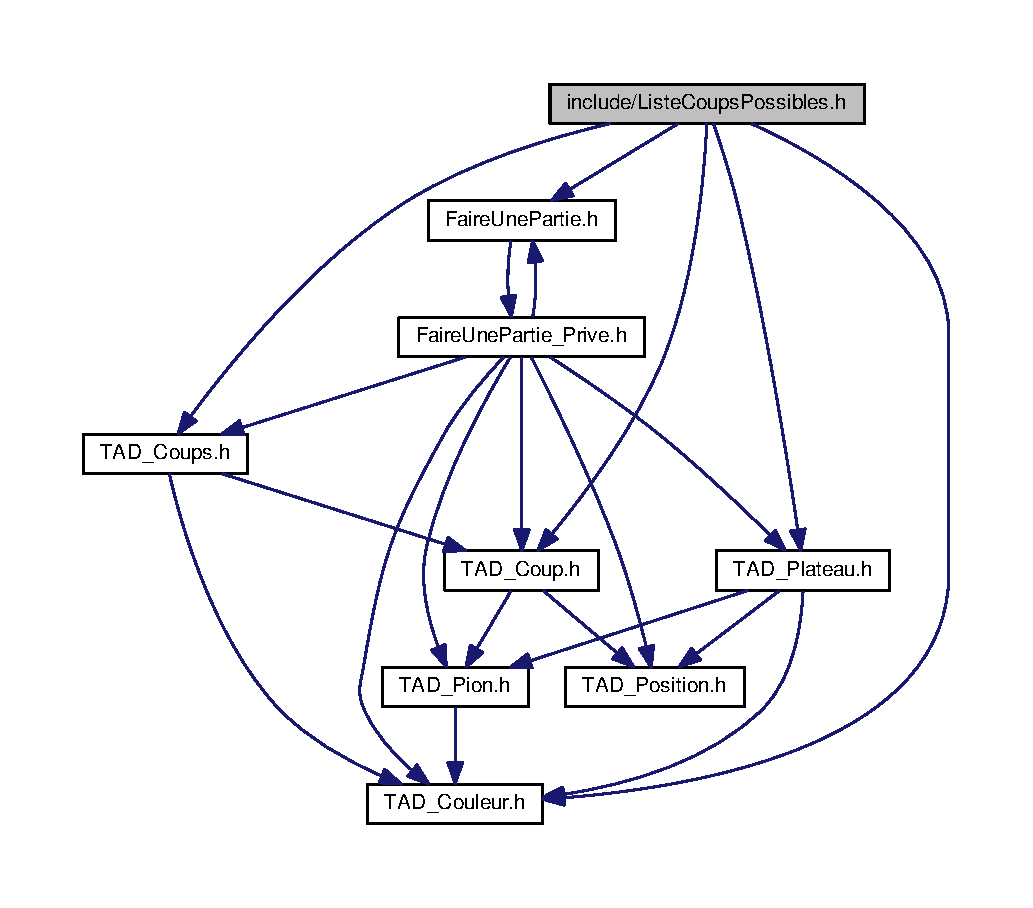
\includegraphics[width=350pt]{_liste_coups_possibles_8h__incl}
\end{center}
\end{figure}
This graph shows which files directly or indirectly include this file\+:
\nopagebreak
\begin{figure}[H]
\begin{center}
\leavevmode
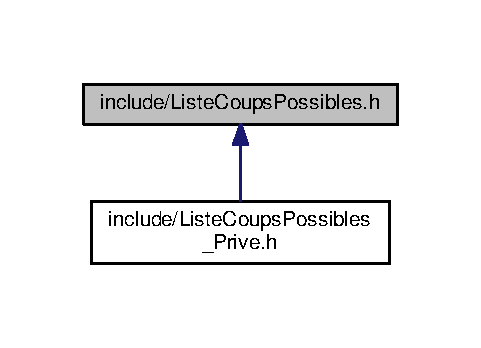
\includegraphics[width=231pt]{_liste_coups_possibles_8h__dep__incl}
\end{center}
\end{figure}
\subsection*{Functions}
\begin{DoxyCompactItemize}
\item 
\hyperlink{struct_coups}{Coups} \hyperlink{_liste_coups_possibles_8h_a870da467e63478902e15f674bc1724dd}{liste\+Coups\+Possibles} (\hyperlink{struct_plateau}{Plateau} plateau, \hyperlink{_t_a_d___couleur_8h_aa304d0ca681f782b1d7735da33037dd7}{Couleur} couleur)
\begin{DoxyCompactList}\small\item\em Fonction qui retourne un ensemble de coups possibles. \end{DoxyCompactList}\item 
void \hyperlink{_liste_coups_possibles_8h_a3c6daf3d4b0cb1741cbbbe43be378350}{copier\+Plateau} (\hyperlink{struct_plateau}{Plateau} plateau\+A\+Copier, \hyperlink{struct_plateau}{Plateau} $\ast$plateau\+Copie)
\begin{DoxyCompactList}\small\item\em Procédure qui copie un plateau sur un autre. \end{DoxyCompactList}\end{DoxyCompactItemize}


\subsection{Detailed Description}
Implantation et signatures des fonctions publiques de Liste\+Coups\+Possibles. 

\begin{DoxyAuthor}{Author}
Groupe 1.\+5 
\end{DoxyAuthor}
\begin{DoxyVersion}{Version}
1.\+0 
\end{DoxyVersion}
\begin{DoxyDate}{Date}
02/12/2015 
\end{DoxyDate}


\subsection{Function Documentation}
\hypertarget{_liste_coups_possibles_8h_a3c6daf3d4b0cb1741cbbbe43be378350}{}\index{Liste\+Coups\+Possibles.\+h@{Liste\+Coups\+Possibles.\+h}!copier\+Plateau@{copier\+Plateau}}
\index{copier\+Plateau@{copier\+Plateau}!Liste\+Coups\+Possibles.\+h@{Liste\+Coups\+Possibles.\+h}}
\subsubsection[{copier\+Plateau}]{\setlength{\rightskip}{0pt plus 5cm}void copier\+Plateau (
\begin{DoxyParamCaption}
\item[{{\bf Plateau}}]{plateau\+A\+Copier, }
\item[{{\bf Plateau} $\ast$}]{plateau\+Copie}
\end{DoxyParamCaption}
)}\label{_liste_coups_possibles_8h_a3c6daf3d4b0cb1741cbbbe43be378350}


Procédure qui copie un plateau sur un autre. 


\begin{DoxyParams}{Parameters}
{\em \hyperlink{struct_plateau}{Plateau}} & plateau\+A\+Copier, le plateau à copier \\
\hline
{\em Plateau$\ast$} & plateau\+Copie, le plateau copié \\
\hline
\end{DoxyParams}
\hypertarget{_liste_coups_possibles_8h_a870da467e63478902e15f674bc1724dd}{}\index{Liste\+Coups\+Possibles.\+h@{Liste\+Coups\+Possibles.\+h}!liste\+Coups\+Possibles@{liste\+Coups\+Possibles}}
\index{liste\+Coups\+Possibles@{liste\+Coups\+Possibles}!Liste\+Coups\+Possibles.\+h@{Liste\+Coups\+Possibles.\+h}}
\subsubsection[{liste\+Coups\+Possibles}]{\setlength{\rightskip}{0pt plus 5cm}{\bf Coups} liste\+Coups\+Possibles (
\begin{DoxyParamCaption}
\item[{{\bf Plateau}}]{plateau, }
\item[{{\bf Couleur}}]{couleur}
\end{DoxyParamCaption}
)}\label{_liste_coups_possibles_8h_a870da467e63478902e15f674bc1724dd}


Fonction qui retourne un ensemble de coups possibles. 


\begin{DoxyParams}{Parameters}
{\em \hyperlink{struct_plateau}{Plateau}} & plateau, le plateau \\
\hline
{\em Couleur} & couleur, couleur du joueur courant \\
\hline
\end{DoxyParams}
\begin{DoxyReturn}{Returns}
\hyperlink{struct_coups}{Coups} 
\end{DoxyReturn}

\hypertarget{_obtenir_coup_humain_8h}{\section{Référence du fichier include/\-Obtenir\-Coup\-Humain.h}
\label{_obtenir_coup_humain_8h}\index{include/\-Obtenir\-Coup\-Humain.\-h@{include/\-Obtenir\-Coup\-Humain.\-h}}
}


Implantation et signatures des fonctions publiques d'Obtenir\-Coup\-Humain.  


{\ttfamily \#include \char`\"{}T\-A\-D\-\_\-\-Coup.\-h\char`\"{}}\\*
{\ttfamily \#include \char`\"{}T\-A\-D\-\_\-\-Plateau.\-h\char`\"{}}\\*
{\ttfamily \#include \char`\"{}T\-A\-D\-\_\-\-Couleur.\-h\char`\"{}}\\*
\subsection*{Fonctions}
\begin{DoxyCompactItemize}
\item 
\hypertarget{_obtenir_coup_humain_8h_a1e296bac5cb22c2d4e6a409f2897f138}{\hyperlink{struct_coup}{Coup} {\bfseries obtenir\-Coup\-Humain} (\hyperlink{struct_plateau}{Plateau} plateau, \hyperlink{_t_a_d___couleur_8h_aa304d0ca681f782b1d7735da33037dd7}{Couleur} couleur)}\label{_obtenir_coup_humain_8h_a1e296bac5cb22c2d4e6a409f2897f138}

\end{DoxyCompactItemize}


\subsection{Description détaillée}
Implantation et signatures des fonctions publiques d'Obtenir\-Coup\-Humain. \begin{DoxyAuthor}{Auteur}
Groupe 1.\-5 
\end{DoxyAuthor}
\begin{DoxyVersion}{Version}
1.\-0 
\end{DoxyVersion}
\begin{DoxyDate}{Date}
02/12/2015 
\end{DoxyDate}

\hypertarget{_obtenir_coup_i_a_8h}{\section{Référence du fichier include/\-Obtenir\-Coup\-I\-A.h}
\label{_obtenir_coup_i_a_8h}\index{include/\-Obtenir\-Coup\-I\-A.\-h@{include/\-Obtenir\-Coup\-I\-A.\-h}}
}


Implantation et signatures des fonctions publiques d'Obtenir\-Coup\-I\-A.  


{\ttfamily \#include \char`\"{}T\-A\-D\-\_\-\-Coup.\-h\char`\"{}}\\*
{\ttfamily \#include \char`\"{}T\-A\-D\-\_\-\-Plateau.\-h\char`\"{}}\\*
{\ttfamily \#include \char`\"{}T\-A\-D\-\_\-\-Couleur.\-h\char`\"{}}\\*
\subsection*{Macros}
\begin{DoxyCompactItemize}
\item 
\hypertarget{_obtenir_coup_i_a_8h_a392b60380bf551a0291ed9547b8fd3f4}{\#define {\bfseries P\-R\-O\-F\-O\-N\-D\-E\-U\-R}~4}\label{_obtenir_coup_i_a_8h_a392b60380bf551a0291ed9547b8fd3f4}

\end{DoxyCompactItemize}
\subsection*{Fonctions}
\begin{DoxyCompactItemize}
\item 
\hypertarget{_obtenir_coup_i_a_8h_a3971fef345e5c70b42dd647b059709e4}{\hyperlink{struct_coup}{Coup} {\bfseries obtenir\-Coup\-I\-A} (\hyperlink{struct_plateau}{Plateau} plateau, \hyperlink{_t_a_d___couleur_8h_aa304d0ca681f782b1d7735da33037dd7}{Couleur} couleur)}\label{_obtenir_coup_i_a_8h_a3971fef345e5c70b42dd647b059709e4}

\end{DoxyCompactItemize}


\subsection{Description détaillée}
Implantation et signatures des fonctions publiques d'Obtenir\-Coup\-I\-A. \begin{DoxyAuthor}{Auteur}
Groupe 1.\-5 
\end{DoxyAuthor}
\begin{DoxyVersion}{Version}
1.\-0 
\end{DoxyVersion}
\begin{DoxyDate}{Date}
02/12/2015 
\end{DoxyDate}

\hypertarget{_t_a_d___couleur_8h}{\section{Référence du fichier include/\-T\-A\-D\-\_\-\-Couleur.h}
\label{_t_a_d___couleur_8h}\index{include/\-T\-A\-D\-\_\-\-Couleur.\-h@{include/\-T\-A\-D\-\_\-\-Couleur.\-h}}
}


Implantation du T\-A\-D Couleur.  


\subsection*{Énumérations}
\begin{DoxyCompactItemize}
\item 
enum \hyperlink{_t_a_d___couleur_8h_aa304d0ca681f782b1d7735da33037dd7}{Couleur} \{ {\bfseries B\-L\-A\-N\-C}, 
{\bfseries N\-O\-I\-R}
 \}
\begin{DoxyCompactList}\small\item\em Le type Couleur représente les deux couleurs possibles. \end{DoxyCompactList}\end{DoxyCompactItemize}
\subsection*{Fonctions}
\begin{DoxyCompactItemize}
\item 
\hyperlink{_t_a_d___couleur_8h_aa304d0ca681f782b1d7735da33037dd7}{Couleur} \hyperlink{_t_a_d___couleur_8h_a22c6d4f8e2727467aeac4243fe67e211}{C\-L\-\_\-blanc} ()
\begin{DoxyCompactList}\small\item\em Fonction qui retourne la couleur 'blanc'. \end{DoxyCompactList}\item 
\hyperlink{_t_a_d___couleur_8h_aa304d0ca681f782b1d7735da33037dd7}{Couleur} \hyperlink{_t_a_d___couleur_8h_a75693b32b99965e0184b03528cc93f0b}{C\-L\-\_\-noir} ()
\begin{DoxyCompactList}\small\item\em Fonction qui retourne la couleur 'noir'. \end{DoxyCompactList}\item 
\hypertarget{_t_a_d___couleur_8h_a978747d86a604d865b71da8e23d7a64b}{\hyperlink{_t_a_d___couleur_8h_aa304d0ca681f782b1d7735da33037dd7}{Couleur} {\bfseries C\-L\-\_\-changer\-Couleur} (\hyperlink{_t_a_d___couleur_8h_aa304d0ca681f782b1d7735da33037dd7}{Couleur} couleur)}\label{_t_a_d___couleur_8h_a978747d86a604d865b71da8e23d7a64b}

\item 
\hypertarget{_t_a_d___couleur_8h_a7e0c6db0576c3036e22c1c1bad67760e}{int {\bfseries C\-L\-\_\-sont\-Egales} (\hyperlink{_t_a_d___couleur_8h_aa304d0ca681f782b1d7735da33037dd7}{Couleur} couleur1, \hyperlink{_t_a_d___couleur_8h_aa304d0ca681f782b1d7735da33037dd7}{Couleur} couleur2)}\label{_t_a_d___couleur_8h_a7e0c6db0576c3036e22c1c1bad67760e}

\end{DoxyCompactItemize}


\subsection{Description détaillée}
Implantation du T\-A\-D Couleur. \begin{DoxyAuthor}{Auteur}
Groupe 1.\-5 
\end{DoxyAuthor}
\begin{DoxyVersion}{Version}
1.\-0 
\end{DoxyVersion}
\begin{DoxyDate}{Date}
02/12/15 
\end{DoxyDate}


\subsection{Documentation des fonctions}
\hypertarget{_t_a_d___couleur_8h_a22c6d4f8e2727467aeac4243fe67e211}{\index{T\-A\-D\-\_\-\-Couleur.\-h@{T\-A\-D\-\_\-\-Couleur.\-h}!C\-L\-\_\-blanc@{C\-L\-\_\-blanc}}
\index{C\-L\-\_\-blanc@{C\-L\-\_\-blanc}!TAD_Couleur.h@{T\-A\-D\-\_\-\-Couleur.\-h}}
\subsubsection[{C\-L\-\_\-blanc}]{\setlength{\rightskip}{0pt plus 5cm}{\bf Couleur} C\-L\-\_\-blanc (
\begin{DoxyParamCaption}
{}
\end{DoxyParamCaption}
)}}\label{_t_a_d___couleur_8h_a22c6d4f8e2727467aeac4243fe67e211}


Fonction qui retourne la couleur 'blanc'. 

\begin{DoxyReturn}{Renvoie}
Couleur 
\end{DoxyReturn}
\hypertarget{_t_a_d___couleur_8h_a75693b32b99965e0184b03528cc93f0b}{\index{T\-A\-D\-\_\-\-Couleur.\-h@{T\-A\-D\-\_\-\-Couleur.\-h}!C\-L\-\_\-noir@{C\-L\-\_\-noir}}
\index{C\-L\-\_\-noir@{C\-L\-\_\-noir}!TAD_Couleur.h@{T\-A\-D\-\_\-\-Couleur.\-h}}
\subsubsection[{C\-L\-\_\-noir}]{\setlength{\rightskip}{0pt plus 5cm}{\bf Couleur} C\-L\-\_\-noir (
\begin{DoxyParamCaption}
{}
\end{DoxyParamCaption}
)}}\label{_t_a_d___couleur_8h_a75693b32b99965e0184b03528cc93f0b}


Fonction qui retourne la couleur 'noir'. 

\begin{DoxyReturn}{Renvoie}
Couleur 
\end{DoxyReturn}

\hypertarget{_t_a_d___coup_8h}{\section{Référence du fichier include/\-T\-A\-D\-\_\-\-Coup.h}
\label{_t_a_d___coup_8h}\index{include/\-T\-A\-D\-\_\-\-Coup.\-h@{include/\-T\-A\-D\-\_\-\-Coup.\-h}}
}


Implantation du T\-A\-D \hyperlink{struct_coup}{Coup}.  


{\ttfamily \#include \char`\"{}T\-A\-D\-\_\-\-Position.\-h\char`\"{}}\\*
{\ttfamily \#include \char`\"{}T\-A\-D\-\_\-\-Pion.\-h\char`\"{}}\\*
\subsection*{Structures de données}
\begin{DoxyCompactItemize}
\item 
struct \hyperlink{struct_coup}{Coup}
\begin{DoxyCompactList}\small\item\em Le type \hyperlink{struct_coup}{Coup} permet de représenter le coup d'un joueur, en regroupant une position (sur le plateau) et un pion. \end{DoxyCompactList}\end{DoxyCompactItemize}
\subsection*{Fonctions}
\begin{DoxyCompactItemize}
\item 
\hyperlink{struct_coup}{Coup} \hyperlink{_t_a_d___coup_8h_ac8bb7df461819f909ecdcc3274d19e7c}{C\-P\-\_\-creer\-Coup} (\hyperlink{struct_position}{Position} position, \hyperlink{struct_pion}{Pion} pion)
\begin{DoxyCompactList}\small\item\em Fonction qui retourne un coup à partir d'une position et d'un pion. \end{DoxyCompactList}\item 
\hyperlink{struct_position}{Position} \hyperlink{_t_a_d___coup_8h_a24f2d3002a9e57f6f5c48182ae6fef24}{C\-P\-\_\-obtenir\-Position\-Coup} (\hyperlink{struct_coup}{Coup} coup)
\begin{DoxyCompactList}\small\item\em Fonction qui retourne la position d'un coup. \end{DoxyCompactList}\item 
\hyperlink{struct_pion}{Pion} \hyperlink{_t_a_d___coup_8h_ab1e3cb35286e02a9bcd37196d6344d91}{C\-P\-\_\-obtenir\-Pion\-Coup} (\hyperlink{struct_coup}{Coup} coup)
\begin{DoxyCompactList}\small\item\em Fonction qui retourne le pion d'un coup. \end{DoxyCompactList}\item 
\hypertarget{_t_a_d___coup_8h_a73a36992b6f1e68628d0f29b26f386d9}{int {\bfseries C\-P\-\_\-sont\-Egaux} (\hyperlink{struct_coup}{Coup} coup1, \hyperlink{struct_coup}{Coup} coup2)}\label{_t_a_d___coup_8h_a73a36992b6f1e68628d0f29b26f386d9}

\end{DoxyCompactItemize}


\subsection{Description détaillée}
Implantation du T\-A\-D \hyperlink{struct_coup}{Coup}. \begin{DoxyAuthor}{Auteur}
Groupe 1.\-5 
\end{DoxyAuthor}
\begin{DoxyVersion}{Version}
1.\-0 
\end{DoxyVersion}
\begin{DoxyDate}{Date}
02/12/15 
\end{DoxyDate}


\subsection{Documentation des fonctions}
\hypertarget{_t_a_d___coup_8h_ac8bb7df461819f909ecdcc3274d19e7c}{\index{T\-A\-D\-\_\-\-Coup.\-h@{T\-A\-D\-\_\-\-Coup.\-h}!C\-P\-\_\-creer\-Coup@{C\-P\-\_\-creer\-Coup}}
\index{C\-P\-\_\-creer\-Coup@{C\-P\-\_\-creer\-Coup}!TAD_Coup.h@{T\-A\-D\-\_\-\-Coup.\-h}}
\subsubsection[{C\-P\-\_\-creer\-Coup}]{\setlength{\rightskip}{0pt plus 5cm}{\bf Coup} C\-P\-\_\-creer\-Coup (
\begin{DoxyParamCaption}
\item[{{\bf Position}}]{position, }
\item[{{\bf Pion}}]{pion}
\end{DoxyParamCaption}
)}}\label{_t_a_d___coup_8h_ac8bb7df461819f909ecdcc3274d19e7c}


Fonction qui retourne un coup à partir d'une position et d'un pion. 


\begin{DoxyParams}{Paramètres}
{\em \hyperlink{struct_position}{Position}} & position \-: la position à affecter au \hyperlink{struct_coup}{Coup} \\
\hline
{\em \hyperlink{struct_pion}{Pion}} & pion \-: le \hyperlink{struct_pion}{Pion} à affecter au \hyperlink{struct_coup}{Coup} \\
\hline
\end{DoxyParams}
\begin{DoxyReturn}{Renvoie}
\hyperlink{struct_coup}{Coup} 
\end{DoxyReturn}
\hypertarget{_t_a_d___coup_8h_ab1e3cb35286e02a9bcd37196d6344d91}{\index{T\-A\-D\-\_\-\-Coup.\-h@{T\-A\-D\-\_\-\-Coup.\-h}!C\-P\-\_\-obtenir\-Pion\-Coup@{C\-P\-\_\-obtenir\-Pion\-Coup}}
\index{C\-P\-\_\-obtenir\-Pion\-Coup@{C\-P\-\_\-obtenir\-Pion\-Coup}!TAD_Coup.h@{T\-A\-D\-\_\-\-Coup.\-h}}
\subsubsection[{C\-P\-\_\-obtenir\-Pion\-Coup}]{\setlength{\rightskip}{0pt plus 5cm}{\bf Position} C\-P\-\_\-obtenir\-Pion\-Coup (
\begin{DoxyParamCaption}
\item[{{\bf Coup}}]{coup}
\end{DoxyParamCaption}
)}}\label{_t_a_d___coup_8h_ab1e3cb35286e02a9bcd37196d6344d91}


Fonction qui retourne le pion d'un coup. 


\begin{DoxyParams}{Paramètres}
{\em \hyperlink{struct_coup}{Coup}} & coup \-: le coup dont on veut le pion \\
\hline
\end{DoxyParams}
\begin{DoxyReturn}{Renvoie}
\hyperlink{struct_coup}{Coup} 
\end{DoxyReturn}
\hypertarget{_t_a_d___coup_8h_a24f2d3002a9e57f6f5c48182ae6fef24}{\index{T\-A\-D\-\_\-\-Coup.\-h@{T\-A\-D\-\_\-\-Coup.\-h}!C\-P\-\_\-obtenir\-Position\-Coup@{C\-P\-\_\-obtenir\-Position\-Coup}}
\index{C\-P\-\_\-obtenir\-Position\-Coup@{C\-P\-\_\-obtenir\-Position\-Coup}!TAD_Coup.h@{T\-A\-D\-\_\-\-Coup.\-h}}
\subsubsection[{C\-P\-\_\-obtenir\-Position\-Coup}]{\setlength{\rightskip}{0pt plus 5cm}{\bf Position} C\-P\-\_\-obtenir\-Position\-Coup (
\begin{DoxyParamCaption}
\item[{{\bf Coup}}]{coup}
\end{DoxyParamCaption}
)}}\label{_t_a_d___coup_8h_a24f2d3002a9e57f6f5c48182ae6fef24}


Fonction qui retourne la position d'un coup. 


\begin{DoxyParams}{Paramètres}
{\em \hyperlink{struct_coup}{Coup}} & coup \-: le coup dont on veut la position \\
\hline
\end{DoxyParams}
\begin{DoxyReturn}{Renvoie}
\hyperlink{struct_coup}{Coup} 
\end{DoxyReturn}

\hypertarget{_t_a_d___coups_8h}{\section{Référence du fichier include/\-T\-A\-D\-\_\-\-Coups.h}
\label{_t_a_d___coups_8h}\index{include/\-T\-A\-D\-\_\-\-Coups.\-h@{include/\-T\-A\-D\-\_\-\-Coups.\-h}}
}


Implantation du T\-A\-D \hyperlink{struct_coups}{Coups}.  


{\ttfamily \#include \char`\"{}T\-A\-D\-\_\-\-Coup.\-h\char`\"{}}\\*
{\ttfamily \#include \char`\"{}T\-A\-D\-\_\-\-Couleur.\-h\char`\"{}}\\*
\subsection*{Structures de données}
\begin{DoxyCompactItemize}
\item 
struct \hyperlink{struct_coups}{Coups}
\begin{DoxyCompactList}\small\item\em Le type \hyperlink{struct_coups}{Coups} permet de représenter un tableau de \hyperlink{struct_coup}{Coup} et le nombre de \hyperlink{struct_coup}{Coup} possibles. \end{DoxyCompactList}\end{DoxyCompactItemize}
\subsection*{Macros}
\begin{DoxyCompactItemize}
\item 
\hypertarget{_t_a_d___coups_8h_a72b7ac89f46d3cb2aa9e9eddb69e7adc}{\#define {\bfseries M\-A\-X\-\_\-\-C\-O\-U\-P\-S}~60}\label{_t_a_d___coups_8h_a72b7ac89f46d3cb2aa9e9eddb69e7adc}

\end{DoxyCompactItemize}
\subsection*{Fonctions}
\begin{DoxyCompactItemize}
\item 
\hypertarget{_t_a_d___coups_8h_aa2ce3e213706ca436cacbda18e34f5c2}{void {\bfseries C\-P\-S\-\_\-creer\-Coups} (\hyperlink{struct_coups}{Coups} $\ast$coups)}\label{_t_a_d___coups_8h_aa2ce3e213706ca436cacbda18e34f5c2}

\item 
void \hyperlink{_t_a_d___coups_8h_af2e7edcec7429d4bdfd2663eb195ecc3}{C\-P\-S\-\_\-ajouter\-Coups} (\hyperlink{struct_coups}{Coups} $\ast$coups, \hyperlink{struct_coup}{Coup} coup)
\begin{DoxyCompactList}\small\item\em Fonction ajoute le \hyperlink{struct_coup}{Coup} coup à la variable coups. \end{DoxyCompactList}\item 
unsigned int \hyperlink{_t_a_d___coups_8h_af1de1eae45bfb41101a8011d0f72557d}{C\-P\-S\-\_\-nb\-Coups} (\hyperlink{struct_coups}{Coups} coups)
\begin{DoxyCompactList}\small\item\em Fonction qui renvoie le nombre de \hyperlink{struct_coups}{Coups} d'une variable de type \hyperlink{struct_coups}{Coups}. \end{DoxyCompactList}\item 
\hyperlink{struct_coup}{Coup} \hyperlink{_t_a_d___coups_8h_a8f108bb6178f13d908dd89acec4efec1}{C\-P\-S\-\_\-ieme\-Coup} (\hyperlink{struct_coups}{Coups} coups, unsigned int i)
\begin{DoxyCompactList}\small\item\em Fonction qui ieme \hyperlink{struct_coup}{Coup} de la variable coups. \end{DoxyCompactList}\end{DoxyCompactItemize}


\subsection{Description détaillée}
Implantation du T\-A\-D \hyperlink{struct_coups}{Coups}. \begin{DoxyAuthor}{Auteur}
Groupe 1.\-5 
\end{DoxyAuthor}
\begin{DoxyVersion}{Version}
1.\-0 
\end{DoxyVersion}
\begin{DoxyDate}{Date}
02/12/15 
\end{DoxyDate}


\subsection{Documentation des fonctions}
\hypertarget{_t_a_d___coups_8h_af2e7edcec7429d4bdfd2663eb195ecc3}{\index{T\-A\-D\-\_\-\-Coups.\-h@{T\-A\-D\-\_\-\-Coups.\-h}!C\-P\-S\-\_\-ajouter\-Coups@{C\-P\-S\-\_\-ajouter\-Coups}}
\index{C\-P\-S\-\_\-ajouter\-Coups@{C\-P\-S\-\_\-ajouter\-Coups}!TAD_Coups.h@{T\-A\-D\-\_\-\-Coups.\-h}}
\subsubsection[{C\-P\-S\-\_\-ajouter\-Coups}]{\setlength{\rightskip}{0pt plus 5cm}void C\-P\-S\-\_\-ajouter\-Coups (
\begin{DoxyParamCaption}
\item[{{\bf Coups} $\ast$}]{coups, }
\item[{{\bf Coup}}]{coup}
\end{DoxyParamCaption}
)}}\label{_t_a_d___coups_8h_af2e7edcec7429d4bdfd2663eb195ecc3}


Fonction ajoute le \hyperlink{struct_coup}{Coup} coup à la variable coups. 


\begin{DoxyParams}{Paramètres}
{\em Coups$\ast$} & coups \-: un tableau de \hyperlink{struct_coups}{Coups} \\
\hline
{\em \hyperlink{struct_coup}{Coup}} & coup \-: le \hyperlink{struct_coup}{Coup} à ajouter à coups \\
\hline
\end{DoxyParams}
\hypertarget{_t_a_d___coups_8h_a8f108bb6178f13d908dd89acec4efec1}{\index{T\-A\-D\-\_\-\-Coups.\-h@{T\-A\-D\-\_\-\-Coups.\-h}!C\-P\-S\-\_\-ieme\-Coup@{C\-P\-S\-\_\-ieme\-Coup}}
\index{C\-P\-S\-\_\-ieme\-Coup@{C\-P\-S\-\_\-ieme\-Coup}!TAD_Coups.h@{T\-A\-D\-\_\-\-Coups.\-h}}
\subsubsection[{C\-P\-S\-\_\-ieme\-Coup}]{\setlength{\rightskip}{0pt plus 5cm}{\bf Coup} C\-P\-S\-\_\-ieme\-Coup (
\begin{DoxyParamCaption}
\item[{{\bf Coups}}]{coups, }
\item[{unsigned int}]{i}
\end{DoxyParamCaption}
)}}\label{_t_a_d___coups_8h_a8f108bb6178f13d908dd89acec4efec1}


Fonction qui ieme \hyperlink{struct_coup}{Coup} de la variable coups. 


\begin{DoxyParams}{Paramètres}
{\em \hyperlink{struct_coups}{Coups}} & coups \-: la variable dont on veut obtenir le ieme \hyperlink{struct_coup}{Coup} \\
\hline
{\em unsigned} & int i \-: indice du \hyperlink{struct_coup}{Coup} à obtenir \\
\hline
\end{DoxyParams}
\begin{DoxyReturn}{Renvoie}
\hyperlink{struct_coup}{Coup} \-: le nombre de \hyperlink{struct_coups}{Coups} 
\end{DoxyReturn}
\hypertarget{_t_a_d___coups_8h_af1de1eae45bfb41101a8011d0f72557d}{\index{T\-A\-D\-\_\-\-Coups.\-h@{T\-A\-D\-\_\-\-Coups.\-h}!C\-P\-S\-\_\-nb\-Coups@{C\-P\-S\-\_\-nb\-Coups}}
\index{C\-P\-S\-\_\-nb\-Coups@{C\-P\-S\-\_\-nb\-Coups}!TAD_Coups.h@{T\-A\-D\-\_\-\-Coups.\-h}}
\subsubsection[{C\-P\-S\-\_\-nb\-Coups}]{\setlength{\rightskip}{0pt plus 5cm}unsigned int C\-P\-S\-\_\-nb\-Coups (
\begin{DoxyParamCaption}
\item[{{\bf Coups}}]{coups}
\end{DoxyParamCaption}
)}}\label{_t_a_d___coups_8h_af1de1eae45bfb41101a8011d0f72557d}


Fonction qui renvoie le nombre de \hyperlink{struct_coups}{Coups} d'une variable de type \hyperlink{struct_coups}{Coups}. 


\begin{DoxyParams}{Paramètres}
{\em \hyperlink{struct_coups}{Coups}} & coups \-: la variable dont on veut compter le nombre de \hyperlink{struct_coups}{Coups} \\
\hline
\end{DoxyParams}
\begin{DoxyReturn}{Renvoie}
unsigned int \-: le nombre de \hyperlink{struct_coups}{Coups} 
\end{DoxyReturn}

%--- End generated contents ---

% Index
\backmatter
\newpage
\phantomsection
\clearemptydoublepage
\addcontentsline{toc}{chapter}{Index}
\printindex

\end{document}
